%\documentclass[10pt,xcolor=table]{beamer}
%\documentclass[notes=only,10pt,xcolor=table]{beamer}
\documentclass[notes, 10pt,xcolor=table]{beamer}

% Use the preamble setting
% Beamer theme
\usetheme[titleformat=allcaps, progressbar=foot,
          titleformat title=allcaps, titleformat subtitle=allcaps,
          titleformat section=smallcaps, titleformat frame=smallcaps]{metropolis}
% Settings to have progress bar at the top
\useoutertheme[subsection=false]{miniframes}
\useinnertheme{circles}
%% \usefonttheme{structurebold}
\usecolortheme{beaver}

% Some change in font colour
\setbeamercolor{normal text}{fg=black, bg=white}
\setbeamercolor{altered text}{fg=black, bg=white}
\setbeamercolor{example text}{fg=black, bg=white}

% Change in the title color
\definecolor{BostonUniRed}{rgb}{0.8, 0.0, 0.0}
\setbeamercolor{frametitle}{fg=BostonUniRed, bg=BostonUniRed!10}

% Add graphics path
\usepackage{graphicx}
\graphicspath{{img/}{clips/}}

\usepackage{booktabs}
\usepackage[scale=2]{ccicons}

\usepackage{pgfplots}
\usepgfplotslibrary{dateplot}

\usepackage{pifont}

% Define graphics for logo
\titlegraphic{%
  \includegraphics[height=.125\textheight]{BostonUni.png} \hfill
  %\includegraphics[height=.125\textheight]{CEL_Logo.eps}
}
% Setting title page to be centered, and add logos at the bottom
\makeatletter
\setbeamertemplate{title page}{
  \begin{minipage}[b][\paperheight]{\textwidth}
    % Centering titles    
    \centering  % <-- Center here
    \vfill%
    \ifx\inserttitle\@empty\else\usebeamertemplate*{title}\fi
    \ifx\insertsubtitle\@empty\else\usebeamertemplate*{subtitle}\fi
    \usebeamertemplate*{title separator}
    \ifx\beamer@shortauthor\@empty\else\usebeamertemplate*{author}\fi
    \ifx\insertdate\@empty\else\usebeamertemplate*{date}\fi
    \ifx\insertinstitute\@empty\else\usebeamertemplate*{institute}\fi
    \vfill
    % Inserting logo
    \ifx\inserttitlegraphic\@empty\else\inserttitlegraphic\fi    
    \vspace*{10mm}
  \end{minipage}
}
\setbeamertemplate{title}{
%  \raggedright%  % <-- Comment here
  \linespread{1.0}%
  \inserttitle%
  \par%
  \vspace*{0.5em}
}
\setbeamertemplate{subtitle}{
%  \raggedright%  % <-- Comment here
  \insertsubtitle%
  \par%
  \vspace*{0.5em}
}
\makeatother

% Manage frame numbering in beamer's appendixes
\usepackage{appendixnumberbeamer}

% URL
\usepackage{hyperref}

% Citation
%\usepackage[backend=bibtex, style=science]{biblatex}
\usepackage[backend=bibtex]{biblatex}
% Hacky fix to citation
\makeatletter
\def\blx@maxline{77}
\makeatother
% Reduce font size for citation
\setbeamerfont{bibliography item}{size=\footnotesize}
\setbeamerfont{bibliography entry author}{size=\footnotesize}
\setbeamerfont{bibliography entry title}{size=\footnotesize}
\setbeamerfont{bibliography entry location}{size=\footnotesize}
\setbeamerfont{bibliography entry note}{size=\footnotesize}
\renewcommand{\footnotesize}{\tiny}

% Change caption font size
\usepackage[font=scriptsize, labelfont=bf]{caption}
\usepackage{subcaption}

% Box around text
\usepackage{tcolorbox}

% For large table in the timeline
\usepackage{chngpage}


% Title and logo
\title{Operating System Energy-Performance Trade-offs towards System Self Optimization}
\subtitle{Dissertation Prospectus}
%\date{\today}
\date{January 24, 2022}
\author{Han Dong}

% Add bibliography file
\bibliography{reference}

\begin{document}
% Make the title
{
% Uncomment the following to dismiss the transparent background crest
\setbeamertemplate{background}{\tikz[remember picture,overlay]\node[opacity=0.04] at (current page.center) {\includegraphics[height=0.8\paperheight,keepaspectratio]{BostonUni_Crest.eps}};}
\maketitle
}

% Setting all titles to be centered
\setbeamertemplate{frametitle}[default][center]

% Table of content
\begin{frame}[plain]{Table of Contents}
  \setbeamertemplate{section in toc}[sections numbered]
  \tableofcontents[hideallsubsections]
\end{frame}

% Section 1
\section{Introduction}

%% TRENDS IN COMPUTING
\begin{frame}
  \frametitle{Trends in computing}
  \only<1>{
  \begin{itemize}
  \item Energy growth in computing.
  \item Hardware increasingly complex, many features packed into it.
  \item Software dedicated to run on a single node within a datacenter.
  \end{itemize}
  }
  \only<2>{
  \begin{itemize}
  \item Energy growth in computing.
  \item Hardware increasingly complex, many features packed into it.
  \item Software dedicated to run on a single node within a datacenter.
  \end{itemize}
  \begin{figure}
    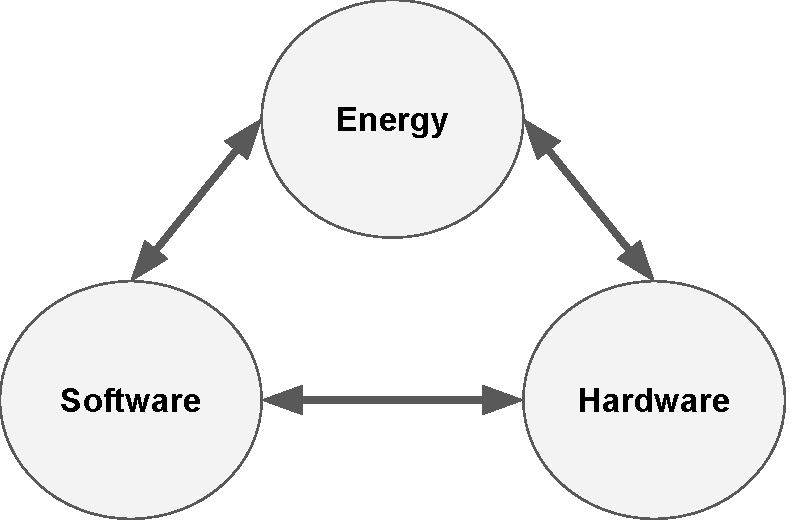
\includegraphics[width=0.65\textwidth]{img/energy-sw-hw-tradeoff.pdf}
    %\caption{Two mantis on a wig.}
  \end{figure}
  }
\end{frame}
%% NOTES
\note{
\begin{itemize}
    \item There are other trends, but I identify these are useful/important to consider with respect to OSes and challenges we face
    \item Relationship between the 3 and questions to be asked in this setup
    \item Point 3 can be exploited to make these things easier
\end{itemize}
}
%%%%%%%%%%%%%%%%%%%%%%%%%%%%

%% ENERGY
\begin{frame}{Energy}
\framesubtitle{Trends in computing}
\begin{columns}
    \begin{column}{.5\textwidth}
        \begin{figure}
            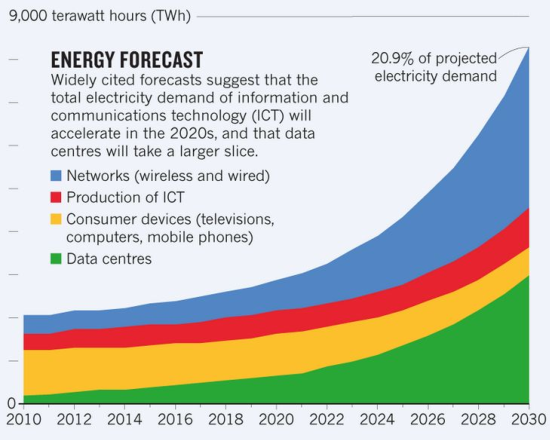
\includegraphics[width=0.9\textwidth]{img/energyuse1.pdf}
            \caption{Nicola Jones, How to stop data centres from gobbling up the world’s electricity, 9/12/2018~\cite{nature1}.}
        \end{figure}
    \end{column}
    \begin{column}{.5\textwidth}
        \begin{figure}
            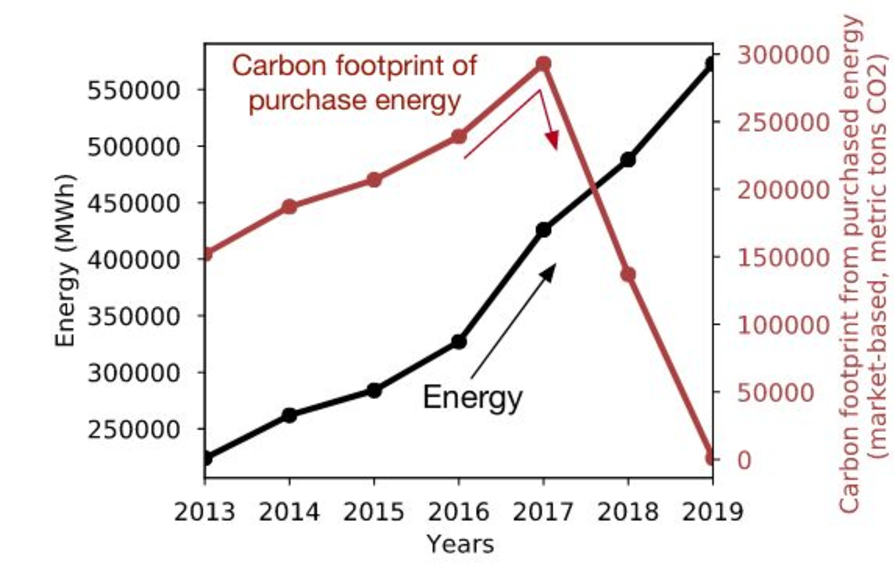
\includegraphics[width=0.9\textwidth]{img/energyuse2.pdf}
            \caption{Udit Gupta et al. Chasing Carbon: The Elusive Environmental Footprint of Computing, 10/28/2020~\cite{gupta2020chasing}.}
        \end{figure}
    \end{column}
    \end{columns}
\end{frame}
\note{
\begin{itemize}
    \item By changing software, exploit more out of existing data center
    \item squeezing more utilization out of existing data center budgets
\end{itemize}
}
%%%%%%%%%%%%%%%%%%%%%%%%%%%%

%% Hardware Complexity
\begin{frame}{Hardware Complexity}
\framesubtitle{Trends in computing}
    \only<1>{
    \begin{itemize}
        \item Hardware logic has grown to accommodate more configurable features:
        \begin{itemize}
            \item Reflect changing application requirements.
            \item Offload work that used to be done by software.
        \end{itemize}
    \end{itemize}
    }
    \only<2>{
    \begin{columns}
      \begin{column}{.4\textwidth}
        \begin{itemize}
        \item Hardware logic has grown to accommodate more configurable features.
        \begin{itemize}
            \item Reflect changing application requirements.
            \item Offload work that used to be done by software.
        \end{itemize}
    \end{itemize}
      \end{column}
      \begin{column}{.6\textwidth}
        \begin{figure}
            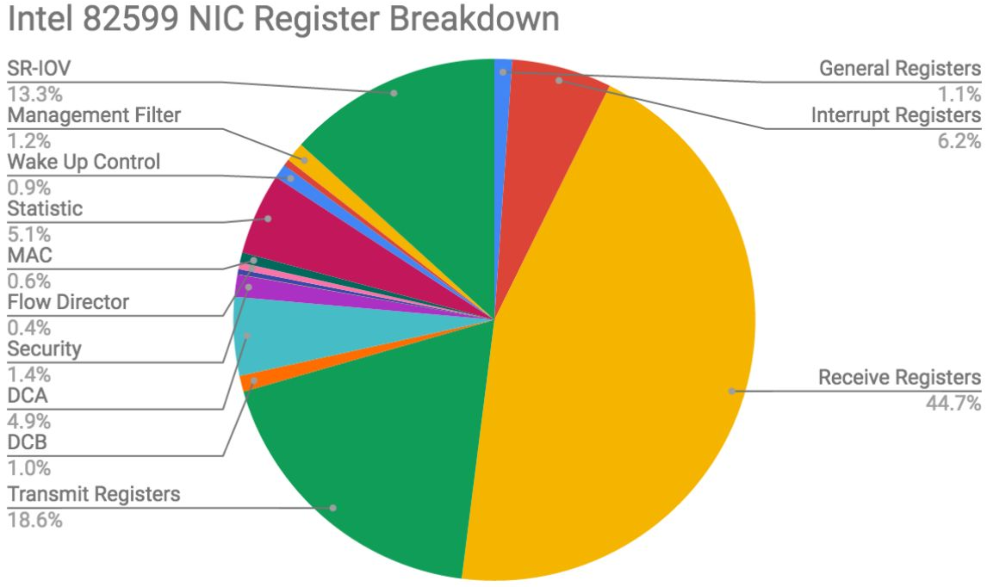
\includegraphics[width=1.0\textwidth]{img/82599_NIC.pdf}
            \caption{Breakdown of table of contents in Intel 82599 10 GbE NIC datasheet~\cite{82599}.}
        \end{figure}
      \end{column}
    \end{columns}
    \note{over 5000 configurable features}
    }
    \only<3>{
    \begin{columns}
      \begin{column}{.4\textwidth}
        \begin{itemize}
        \item Device drivers have grown in complexity to drive these features.
        \item Effectively using these features is dependent on algorithms provided by manufacturers.
        % \begin{itemize}
        %     \item Software shielded away from needing to manage this sort of complexity.
        % \end{itemize}
    \end{itemize}
      \end{column}
      \begin{column}{.6\textwidth}
        \begin{figure}
            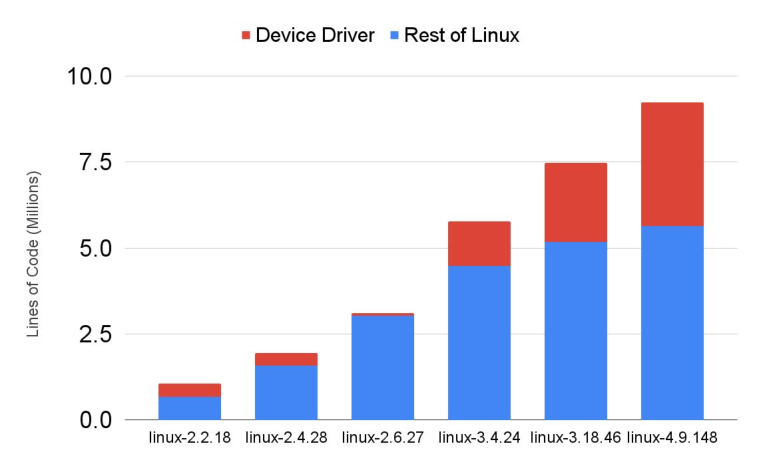
\includegraphics[width=1.0\textwidth]{img/devicedriverloc.pdf}
            \caption{Lines of code measured from Linux kernel in last 10 years using SLOCCount~\cite{sloccount}.}
        \end{figure}
      \end{column}
    \end{columns}
    }
\end{frame}
\note{
\begin{itemize}
    \item Example features: security, checksum offloading, batching, packet coalescing
    \item Some features offloaded used to be in SW
    \item Software shielded away from needing to manage this sort of complexity.
\end{itemize}
}
%%%%%%%%%%%%%%%%%%%%%%%%%%%%

%% Software Dedication
\begin{frame}{Software Dedication}
\framesubtitle{Trends in computing}
    \only<1>{
    \begin{itemize}
        \item Data center aggregation of all compute with massive amounts of hardware nodes:
        \begin{itemize}
            \item[\ding{212}] Dedication of entire nodes to meet application demand.
        \end{itemize}
    \end{itemize}
    }
    \only<2>{
    \begin{itemize}
        % \item Data center aggregation of all compute with massive amounts of hardware:
        % \begin{itemize}
        %     \item[\ding{212}] Dedication of entire nodes to meet application demand.
        % \end{itemize}
        % \vspace{0.5cm}
        \item Facebook's cluster management system (\textbf{Twine}~\cite{twine}): 
        \begin{itemize}
            \item Elastically scale clusters of many small machines (1 CPU, 64 Gb RAM).
            \item Applications use containers (rather than VMs) for deployment.
            \item \textbf{Per-node customizations} such as NIC settings, kernel versions, sysctl, filesystems, etc.
        \end{itemize}
    \end{itemize}
    }
    \only<3>{
    \begin{itemize}
        \item In academia, renewed interest in building per-application systems~\cite{ix, mica, zygos, shenango, bmcmcd, dynsleep, 10.1145/3132747.3132764, 10.5555/2387880.2387894, segcache, stackmap, seuss, arrakis, rumpkernel, unikernels, aliraza}, such as library OSes, unikernels, kernel-bypass techniques, etc. %, mostly written using modern programming languages such as C/C++, Python, Rust, golang, etc.
        \begin{itemize}
            \item[\ding{212}] Mostly focused on performance, energy efficiency is a largely un-explored.
        \end{itemize}
    \end{itemize}
    }
\end{frame}
\note{
\begin{itemize}
    \item 
\end{itemize}
}
%%%%%%%%%%%%%%%%%%%%%%%%%%%%

%%

%%%%%%%%%%%%%%%%%%%%%%%%%%%%

\begin{frame}
  \frametitle{Unusual layout frame}
  \begin{columns}
    \begin{column}{.44\textwidth}
      \begin{figure}[t]
        \includegraphics[width=0.8\textwidth]{cat}
        \caption{A picture of a cat in a pot hole\footnotemark[1].}
      \end{figure}
    \end{column}
    \begin{column}{.60\textwidth}
      Observations:
        \begin{itemize}
        \item There is a cat.
        \item It looks like it's stuck in a pot hole.
        \end{itemize}
    \end{column}
  \end{columns}

  You can also split things into two columns and arrange them as so.
  
  \vspace{0.8cm}
  % Quick fix to citation for subfigures
  \sbox1{\hbox{\footfullcite[1]{cat}}}
\end{frame}

% Section 2
\section{Methodology}
\begin{frame}
  \frametitle{How to perform research}
  \begin{figure}
    \includegraphics[width=0.5\textwidth]{hedgehog}
    \caption{Hedgehog posing in a tiny kayak.}
  \end{figure}
  \vspace{-0.4cm}
  \begin{itemize}
  \item This is a picture of a happy hedgehog.
  \item You can even cite where this hedgehog is from \footfullcite{hedgehog}.
  \end{itemize}
  \vspace{0.15cm}
\end{frame}

\begin{frame}
  \frametitle{Concurrent vs Information-passing}
  \begin{columns}
    \begin{column}{0.5\textwidth}
      \begin{figure}
        \includegraphics[width=0.45\textwidth]{gecko}
        \caption{Gecko strumming a leaf\footnotemark[2].}
      \end{figure}
      \begin{itemize}
      \item He pulled out his guitar:
      \item `Anyway, here's Wonderwall.'
      \end{itemize}
    \end{column}
    \begin{column}{0.5\textwidth}
      \begin{figure}
        \includegraphics[width=0.45\textwidth]{eagle}
        \caption{Bald eagle over ice\footnotemark[3].}
      \end{figure}
      \begin{itemize}
      \item `\textit{When will my reflection shows...}'
      \item `\textit{...who I am, inside}.'
      \end{itemize}      
    \end{column}    
  \end{columns}
  \vspace{0.25cm}
  % Again, fix for the citation at the bottom
  \sbox1{\hbox{\footfullcite[2]{gecko}}}
  \sbox1{\hbox{\footfullcite[3]{eagle}}}
\end{frame}


% Results
\section{Results}
\begin{frame}
  \frametitle{Computer models and calibration}
  \begin{itemize}
  \item Some results here...
  \item Some results there...
  \item And happy dancing mantis!
  \end{itemize}  
  \begin{figure}
    \includegraphics[width=0.65\textwidth]{mantis}
    \caption{Two mantis on a wig.}
  \end{figure}
\end{frame}

% Conclusion and Further work
\section{Conclusion and Further work}
\begin{frame}
  \frametitle{Remarks}
  \begin{itemize}
  \item The first goal is working hard.
  \item The second goal is working a bit harder.
  \item The most important goal is, however, having fun.
  \item And you also get called a doctor by the end of it.
  \end{itemize}
\end{frame}

% Typically asked - time line for the project
\begin{frame}
  \frametitle{Timeline for the project}
\begin{table}[tp]
  \caption{Timeline for the project.}
  \label{table:timeline}
  % If you need to adjust the table when it gets too large
  \begin{adjustwidth}{-0.15in}{0.0in}
    \centering
    \footnotesize
    \begin{tabular}{|l|l|l|l|l|l|l|l|l|}
      \hline
      & \textbf{Q3-2019}                  & \textbf{Q4-2019}                 & \textbf{Q1-2020} & \textbf{Q2-2020} & \textbf{Q3-2020} & \textbf{Q4-2020}      & \textbf{Q1-2021}      & \textbf{Q2-2021}     \\ \hline
      Wake up           & \multicolumn{2}{l|}{\cellcolor[HTML]{34FF34}{\color[HTML]{000000} }} &                  &                  &                  &                       &                       &                      \\ \hline
      Get up           & \multicolumn{2}{l|}{\cellcolor[HTML]{38FFF8}{\color[HTML]{000000} }} &                  &                  &                  &                       &                       &                      \\ \hline
      Dress up &                                   & \multicolumn{2}{l|}{\cellcolor[HTML]{3531FF}}       &                  &                  &                       &                       &                      \\ \hline
      Breakfast and coffee          &                                   &                                  & \multicolumn{3}{l|}{\cellcolor[HTML]{6200C9}}          &                       &                       &                      \\ \hline
      Work        &                                   &                                  & \multicolumn{3}{l|}{\cellcolor[HTML]{F8A102}}          &                       &                       &                      \\ \hline
      Gym    &                                   &                                  &                  &                  & \multicolumn{3}{l|}{\cellcolor[HTML]{FD6864}}                    &                      \\ \hline
      Home                  &                                   &                                  &                  &                  &                  & \multicolumn{3}{l|}{\cellcolor[HTML]{CB0000}{\color[HTML]{000000} }} \\ \hline
    \end{tabular}    
  \end{adjustwidth}
\end{table}  
\end{frame}

% A thank you slide
\begin{frame}{\Large Thank you for your attention!}
  \centering \Large Any questions?
\end{frame}

\begin{frame}
    \printbibliography
\end{frame} 
 
\end{document}
